\begin{frame}{Properties of the 1-d ellipsoid}

\begin{columns}[T]

\begin{column}[T]{0.36\textwidth}
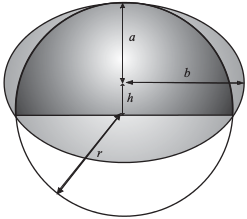
\includegraphics[scale=0.45]{Images/EllipsoidGeometry}
\end{column}

\begin{column}[T]{0.6\textwidth}
\begin{exampleblock}{}
\small Ellipsoid $\varepsilon_n$, containing the bubble shape in $E^n$, has parameters \\ $\displaystyle b=\left(\alpha+\frac{1}{\alpha}\right)\frac{r}{2},\quad h=\left(1-\frac{1}{\alpha^2}\right)\frac{r}{2}$, \\ where $\displaystyle\alpha=\frac{b}{a}$ and $r$ is the radius of the ball $S_n$.
\end{exampleblock}
\end{column}

\end{columns}

\begin{exampleblock}{}
\small If <<to stretch>> the space with factor $\alpha$ in the direction of the semiaxes $a$, the ellipsoid $\varepsilon_n$ will be a ball in the new space.
\end{exampleblock}

\begin{block}{The ratio of the volume of the ellipsoid $\varepsilon_n$ to the volume of a ball $S_n$ is}
$$
q(n)=\frac{vol(\varepsilon_n)}{vol(S�_n)}=\frac{1}{\alpha}\left(\frac{b}{r}\right)^n=\frac{1}{\alpha}\left(\frac{1}{2}\left(\alpha+\frac{1}{\alpha}\right)\right)^n.
$$
\end{block}

\end{frame}